\section{A Distribution Matching Perspective on Vector Quantization}\label{sec:understanding}

This section introduces a novel distributional perspective for understanding vector quantization. By defining three principled criteria for VQ evaluation, we provide empirical and theoretical evidence that aligning feature and code vector distributions  yields a near-optimal VQ solution.

\subsection{An Overview of Vector Quantization}\label{sec:overview vq}
As a core component of visual tokenizers~\cite{Oord2017NeuralDR,Lee2022AutoregressiveIG,Tian2024VisualAM}, VQ acts as a compressor that discretizes continuous latent features into discrete visual tokens by mapping them to the nearest code vectors within a learnable codebook. 

\begin{wrapfigure}[9]{r}{0.50\textwidth}
\small
\vspace{-8mm}
\begin{center}
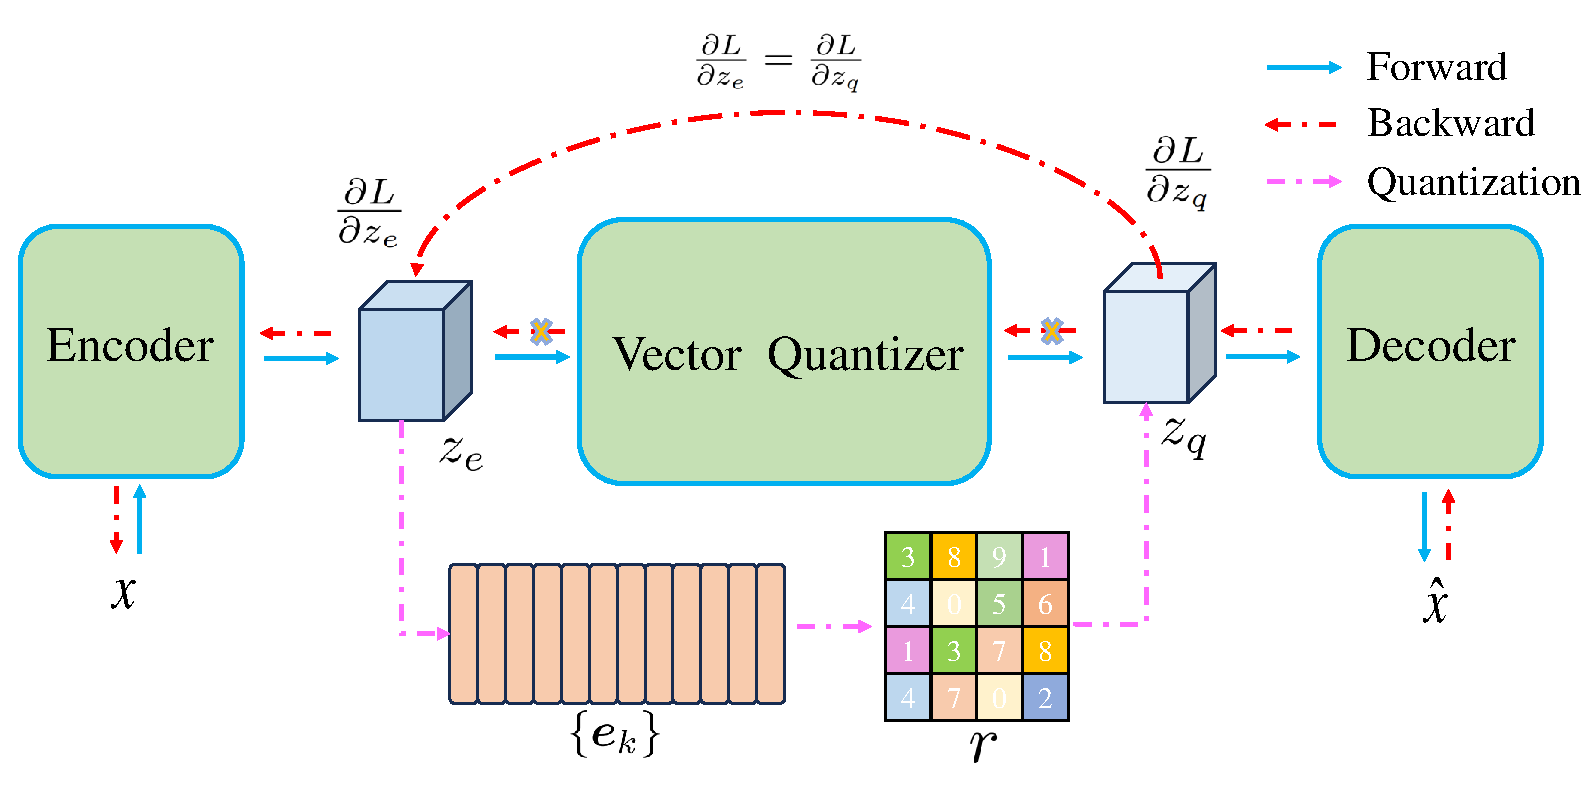
\includegraphics[width=0.48\textwidth]{figs/architecture/VQ.pdf}
\vspace{-4mm}
\caption{\small{The illustration of VQ.}}
\label{fig:vq model}
\end{center}
\end{wrapfigure} 
Figure~\ref{fig:vq model} illustrates the classic VQ process~\cite{Oord2017NeuralDR}, which consists of an encoder $E(\cdot)$, a decoder $D(\cdot)$, and an updatable codebook  $\{\m e_k\}_{k=1}^{K} \in \mathbb{R}^d$ containing a finite set of
code vectors. Here, $K$ denotes the codebook size and $d$ the code vector dimension. Given an image $\bm{x}\in \mathbb{R}^{H\times W \times 3}$, the goal is to derive a spatial collection of codeword IDs $r \in \mathbb{N}^{h\times w}$ as image tokens. This is achieved by encoding the image to obtain $\bm{z}_e = E(\bm{x}) \in \mathbb{R}^{h\times w \times d}$, followed by a spatial quantizer $\mathcal{Q}(\cdot)$ that maps each spatial feature $\bm{z}_{e}^{ij}$ to its nearest code vector $\bm{e}_k$:
\begin{equation}
r^{ij} = \argmin_{k} \|\bm{z}_{e}^{ij} - \bm{e}_k\|_2^2.
\end{equation}
The resulting tokens retrieve the corresponding codebook entries $ \bm{z}_q^{ij} = \mathcal{Q}(\bm{z}_{e}^{ij}) = \bm{e}_{r^{ij}}$, which are then passed through the decoder to reconstruct the image as $\bm{\hat{x}} = D(\bm{z}_q)$. Despite its widespread adoption in visual tokenization, representation learning, and high-fidelity image synthesis~\cite{Esser2020TamingTF}, VQ still faces two key challenges: training instability and codebook collapse.

\paragraph{Training Instability}
This issue arises because during backpropagation, the gradient of $\bm{z}_q$ cannot flow directly to $\bm{z}_e$ due to the non-differentiable function $\mathcal{Q}$. To optimize the encoder's parameters, VQ-VAE~\cite{Oord2017NeuralDR} employs the straight-through estimator~(STE)~\cite{Bengio2013EstimatingOP}, which copies gradients from $\bm{z}_q$ to $\bm{z}_e$. However, this approach carries significant risks, especially when $\bm{z}_q$ and $\bm{z}_e$ are far apart. In such cases, the gradient gap can grow substantially, destabilizing training\footnote{Appendix~\ref{appendix:gradient gap quantization error} details the gradient-quantization relationship.}. In this work, we tackle the training instability challenge from a distributional viewpoint. This perspective highlights that training instability is not merely an implementation artifact, but a consequence of systematic mismatch between feature and code distributions.

%%%%%%%%%%%%%%%%%%%%%%%%%%%%%%%%%
%%%%%%%Codebook collapse%%%%%%%%%
%%%%%%%%%%%%%%%%%%%%%%%%%%%%%%%%
\paragraph{Codebook Collapse} 
Codebook collapse occurs when only a small subset of code vectors receives gradients, while most remain unrepresentative and unupdated~\cite{Dhariwal2020JukeboxAG,Yu2021VectorquantizedIM,Lee2022AutoregressiveIG,Zheng2023OnlineCC}. Researchers have proposed solutions such as improved codebook initialization~\cite{Zhu2024ScalingTC}, reinitialization strategies~\cite{Dhariwal2020JukeboxAG,Williams2020HierarchicalQA}, and classical clustering algorithms like $k$-means~\cite{Bradley1998RefiningIP} and $k$-means++\cite{Arthur2007kmeansTA} for codebook optimization~\cite{Razavi2019GeneratingDH,Zheng2023OnlineCC}. Beyond deterministic approaches that select the best-matching token, stochastic quantization strategies have also been explored~\cite{Zhang2023RegularizedVQ,Ramesh2021ZeroShotTG,Takida2022SQVAEVB}. However, these methods still exhibit low code vector utilization, particularly with large codebook sizes $K$~\cite{Zheng2023OnlineCC,Mentzer2023FiniteSQ}. In this paper, we address this issue via distributional matching between feature and code vectors.

%%%%%%%%%%%%%%%%%%%%%%%%%%%%%%%%%%%%%%%
%%%%%%%%%%Evaluation Criteria%%%%%%%%%%
%%%%%%%%%%%%%%%%%%%%%%%%%%%%%%%%%%%%%%%
\subsection{Evaluation Criteria}\label{sec:distributional formulation}
While these quantities have appeared individually in prior work, we emphasize that considering them jointly provides a unified lens for analyzing both optimization stability and codebook collapse.

Given feature vectors $\{\bz_i\}_{i=1}^N$ from feature distribution $\mathcal{P}_A$ and code vectors $\{\be_k\}_{k=1}^K$ sampled from codebook distribution $\mathcal{P}_B$, vector quantization involves finding the nearest, and thus most representative, code vector for each feature: 
\begin{align}
\bz_i'=\argmin_{\be\in\{\be_k\}}\norm{\bz_i-\be}.
\end{align}
Each original feature vector $\bz_i$ is then quantized to $\bz_i'$. We denote the index of the selected code vector for the $i$-th feature as $r_i$, such that $\bm{z}'_i = \bm{e}_{r_i}$.
We next introduce three key criteria to evaluate this process.



\begin{proper}[Quantization Error]\label{criteria:qe} 
The quantization error measures the average distortion introduced and is defined as:
\vspace{-1.0ex}
\begin{align}
\cE(\{\be_k\};\{\bz_i\})=\frac{1}{N}\sum_{i}\norm{\bz_i-\bz_i'}^2.
\end{align}
\end{proper}
A smaller $\cE$ signifies a more accurate quantization of the original feature vectors. 
Beyond this geometric interpretation, $\cE$ is also directly linked to training stability. 
As formally derived in Appendix~\ref{appendix:gradient gap quantization error}, the gradient discrepancy $\mathcal{G}_i$ for a feature $\bz_i$ introduced by the straight-through estimator (STE) is theoretically bounded by its distance to the code vector:
\begin{equation}
    \mathcal{G}_i \le \| \mathbf{H} \|_2 \cdot \| \bz_i-\bz_i' \|,
\end{equation}
where $\mathbf{H} = \left.\frac{\partial^2 \mathcal{L}}{\partial x^2}\right|_{x=\bz_i'}$ 
denotes the Hessian of the overall training loss $\mathcal{L}$ with respect to the latent input,
evaluated at the quantized code $\bz_i'$, characterizing the local curvature of the loss landscape.
%where $\mathbf{H}$ denotes the Hessian of the decoder with respect to its input. 
Since $\cE$ is the mean squared magnitude of the term $\| \bz_i-\bz_i' \|$, minimizing $\cE$ explicitly tightens this bound. This ensures that the approximated gradients remain faithful to the true gradients, effectively mitigating the gradient mismatch that causes training instability.

\begin{proper}[Codebook Utilization Rate]\label{criteria:cu} The codebook utilization rate is the fraction of code vectors used in VQ
\begin{align}
\mathcal{U}(\{\bm{e}_k\};\{\bm{z}_i\}) 
= \frac{1}{K} \sum_{k=1}^K \mathbf{1}\left(k \in \{ r_i \}_{i=1}^N \right),
\end{align}
\end{proper}
where the indicator evaluates to 1 if code vector $\be_k$ is selected by at least one feature. 

A higher $\cU$ reduces the risk of codebook collapse. Ideally, $\cU$ should reach 100\%, meaning all code vectors are utilized. As discussed in Appendix~\ref{appendix:explanation on criterions}, $\cU$ measures only the \emph{completeness} of codebook utilization and cannot evaluate the degree of collapse. This motivates introducing the codebook perplexity criterion.

\begin{proper}[Codebook Perplexity]\label{criteria:cp} The codebook perplexity measures the uniformity of codebook utilization in VQ
\begin{align}
\mathcal{C}(\{\be_k\};\{\bz_i\}) = \exp(-\sum_{k=1}^{K} p_k \log p_k),
\end{align} 
\end{proper}
where $p_k =\frac{1}{N}\sum_{i=1}^N\one(\bz_i'=\be_k)$. A higher $\mathcal{C}$ indicates more uniform selection of code vectors in VQ. Ideally, $\mathcal{C}$ reaches its maximum at $\mathcal{C}_{0} = \exp(-\sum_{k=1}^{K} \frac{1}{K} \log \frac{1}{K})=K$ when code vectors are completely uniformly utilized. Thus, as a complement to Criterion~\ref{criteria:cu}, $\cU$ combined with $\mathcal{C}$ effectively evaluates codebook collapse.

We refer to $(\cE, \cU, \mathcal{C})$ as the criterion triple. When comparing extreme cases of distributional match and mismatch shown in Figure~\ref{fig:distributional match}, we find that distributional matching significantly outperforms mismatching across all three criteria. Using this triple, we can analyze the benefits of distribution matching more systematically.

\paragraph{Quantization Error vs. Codebook Utilization Rate}
Quantization error ($\cE$) is a more fundamental objective than codebook utilization ($\cU$) in VQ. We theoretically show in \cite{Fang2026UnifyingView} that minimizing $\cE$ necessarily induces full codebook utilization, whereas the converse does not hold. This hierarchical relationship suggests treating $\cE$ as the primary optimization target, with $\cU$ serving as a complementary metric to monitor coverage.

\paragraph{Remark} Notably, $\cE$ is sensitive to the variance of the latent feature distribution (Appendix~\ref{appendix:Impact of Distribution Variance}). Consequently, direct comparisons of raw $\cE$ values across latent spaces with different variances can be misleading. To fairly evaluate quantization methods via criterion triple, all comparisons should be made under identical latent distributions.

%\paragraph{Quantization Error vs. Codebook Utilization Rate}
%Quantization error ($\cE$) constitutes a more fundamental objective than codebook utilization ($\cU$) in vector quantization. As theoretically established in \cite{Fang2026UnifyingView}, minimizing $\cE$ necessarily leads to full codebook utilization ($\cU = 100\%$), whereas the reverse is not guaranteed. This hierarchical relationship implies that $\cE$ should be regarded as the primary optimization target, with $\cU$ serving as a complementary metric to monitor codebook coverage.


%%%%%%%%%%%%%%%%%%%%%%%%%%%%%%%%%%%%%%%%%%%%%
%%%%%%%%%%%Distribution Matching%%%%%%%%%%%%%
%%%%%%%%%%%%%%%%%%%%%%%%%%%%%%%%%%%%%%%%%%%%%



\subsection{The Effects of Distribution Matching} \label{sec:effects of distribution matching}
We conduct a deliberately simple synthetic experiment to isolate the geometric effects of distribution mismatch (see details in Appendix~\ref{appendix:details part1}).
% We conduct a simple synthetic experiment to provide intuitive insights (see details in Appendix~\ref{appendix:details part1}).
Specifically, we assume that $\mathcal{P}_A$ and $\mathcal{P}_B$ are uniform distributions within two distinct disks, as shown in Figure~\ref{fig:criterion triple analysis}. We sample feature vectors $\{\bz_i\}_{i=1}^N$ from the red disk and code vectors $\{\be_k\}_{k=1}^K$ from the green circle. The criterion triple $(\cE, \cU, \mathcal{C})$ is calculated by Criteria~\ref{criteria:qe} to~\ref{criteria:cp}.

We examine two cases. The \underline{first} involves disks with identical radii but different centers. As shown in Figures~\ref{fig:diagram 1 group 1} to~\ref{fig:diagram 4 group 1}, when the centers move closer, the criterion triple improves toward optimal values. Specifically, $\cE$ decreases from 1.19 to 0.05, $\cU$ rises from 2\% to 100\%, and $\mathcal{C}$ increases from 3.8 to 344.9. The \underline{second} case shows distributions with identical centers but different radii. When the codebook support lies within the feature support (Figures~\ref{fig:diagram 1 group 2} and~\ref{fig:diagram 2 group 2}), $\cE$ is larger, $\cU$ slightly lower, and $\mathcal{C}$ smaller compared to the aligned distributions in Figure~\ref{fig:diagram 4 group 1}. When the codebook support extends beyond the feature support, $\cE$ increases modestly while $\cU$ and $\mathcal{C}$ drop significantly (Figures~\ref{fig:diagram 3 group 2} and~\ref{fig:diagram 4 group 2}). Detailed explanations are provided in Appendix~\ref{appendix:prototypical study}.

Overall, VQ achieves the optimal criterion triple when feature and codebook distributions are identical. This is further supported by quantitative analyses in Appendix~\ref{appendix:supplementary comprehensive quantitative analyses}.

%We conduct a simple synthetic experiment to provide intuitive insights (See experimental details in Appendix~\ref{appendix:details part1}). 
%Specifically, we assume that the distributions $\mathcal{P}_A$ and $\mathcal{P}_B$ are uniform distributions confined within two distinct disks, as depicted in Figure~\ref{fig:criterion triple analysis}. We then sample a set of feature vectors $\{\bz_i\}_{i=1}^N$ uniformly from the red disk, and a set of code vectors $\{\be_k\}_{k=1}^K$ uniformly from the green circle. The criterion triple $(\cE, \cU, \mathcal{C})$ is then calculated based on the definitions in Criteria~\ref{criteria:qe} to~\ref{criteria:cp}.

%We examine two cases. The first involves two disks with identical radii but different centers. As shown in Figures~\ref{fig:diagram 1 group 1} to~\ref{fig:diagram 4 group 1}, when the centers of the disks move closer together, the criterion triple improves toward optimal values. Specifically, $\cE$ decreases from 1.19 to 0.05, $\cU$ rises from $2\%$ to $100\%$, and $\mathcal{C}$ increases from 3.8 to 344.9.

%The second case shows two distributions with identical centers but different radii. When the codebook distribution's support lies within the feature distribution's support (as shown in Figures~\ref{fig:diagram 1 group 2} and~\ref{fig:diagram 2 group 2}), it results in a notably larger $\cE$, slightly lower $\cU$, and significantly smaller $\mathcal{C}$ compared to the aligned distributions shown in Figure~\ref{fig:diagram 4 group 1}. Conversely, when the codebook distribution's support extends beyond the feature distribution's support, $\cE$ shows a modest increase while both $\cU$ and $\mathcal{C}$ decrease significantly, as illustrated in Figures~\ref{fig:diagram 3 group 2} and~\ref{fig:diagram 4 group 2}. We provide detailed explanations of these experimental results in Appendix~\ref{appendix:prototypical study}. 

%From both cases, we can conclude that the VQ achieves the optimal criterion triple when the feature and codebook distributions are identical. This observation will be further supported by more quantitative analyses in Appendix~\ref{appendix:supplementary comprehensive quantitative analyses}.




%Additionally, we conduct experiments to investigate the criterion triple by varying the covariance matrix. We sample a set of feature vectors $\{\bz_i\}_{i=1}^N$ from the distribution $\mathcal{N}(\bm 0, \m \mathbb{I}_d)$ and a corresponding set of code vectors $\{\be_k\}_{k=1}^K$ from $\mathcal{N}(\bm 0, \sigma^2 \m \mathbb{I}_d)$, where $\sigma$  is selected from $\{ 1, 2, 3, 4, 5, 6\}$. The results for the criterion triple are shown in Figures~\ref{fig:gaussian_codebooksize_sigma_error} to~\ref{fig:gaussian_featuresize_sigma_error}, Figures~\ref{fig:gaussian_codebooksize_sigma_utilization} to~\ref{fig:gaussian_featuresize_sigma_utilization}, and Figures~\ref{fig:gaussian_codebooksize_sigma_perplexity} to~\ref{fig:gaussian_featuresize_sigma_perplexity}. When $\sigma = 1$, indicating identical distributions between $\mathcal{P}_A$ and $\mathcal{P}_B$, all three evaluation criteria reach their optimal values: the lowest $\cE$, highest $\cU$, and largest $\mathcal{C}$ across all tested values of $K, d, N$. This result corroborates our earlier findings.

\begin{figure*}[!t]
    \vspace{-2mm}
	\centering
	\subfloat[$(1.19, 2\%, 3.8)$]{ 
		\label{fig:diagram 1 group 1}  
		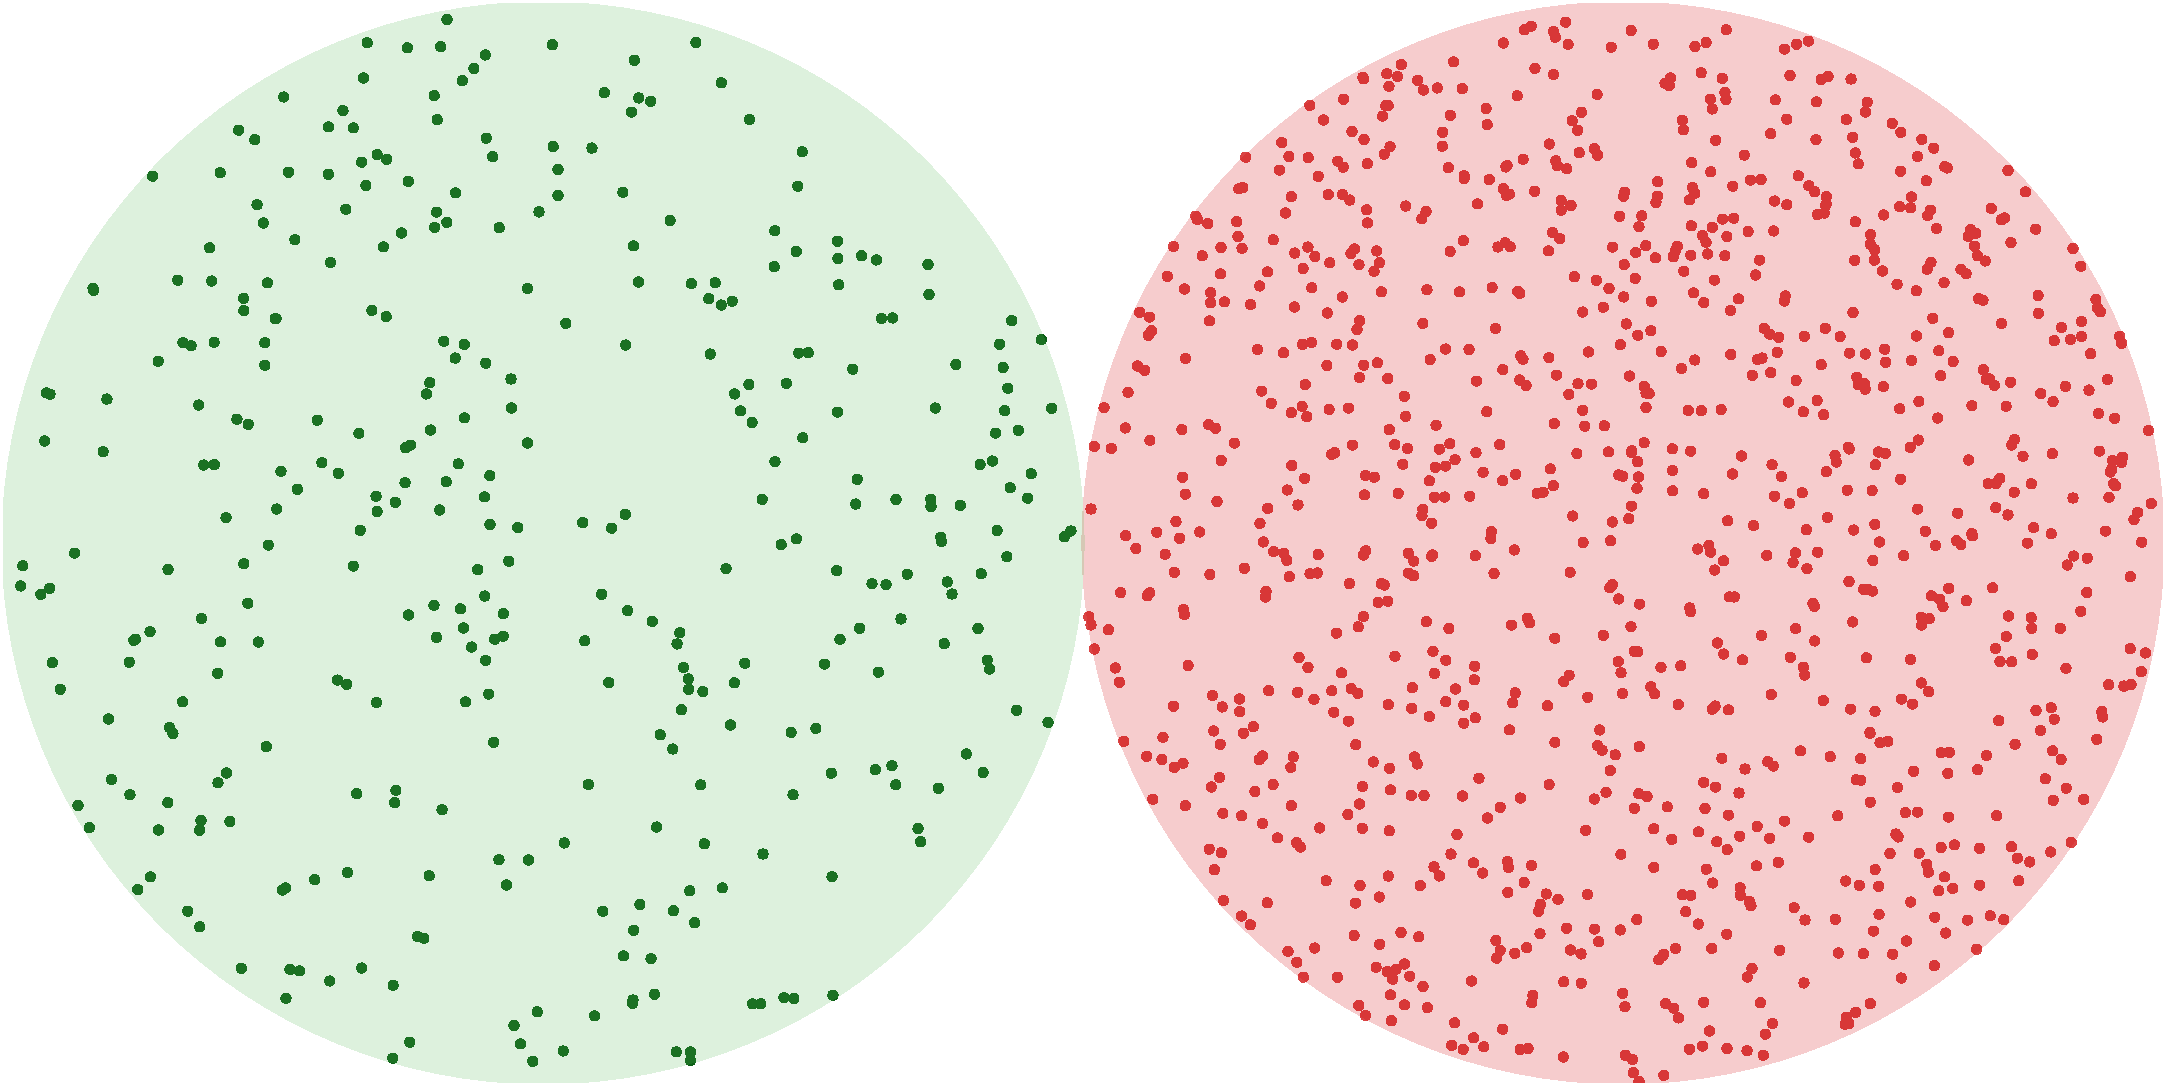
\includegraphics[width=0.22\textwidth]{figs/diagram/Quantative_Simul_Mean=-0.6.pdf}}
	\subfloat[$(0.70, 20.8\%, 16.5)$]{
		\label{fig:diagram 2 group 1}
		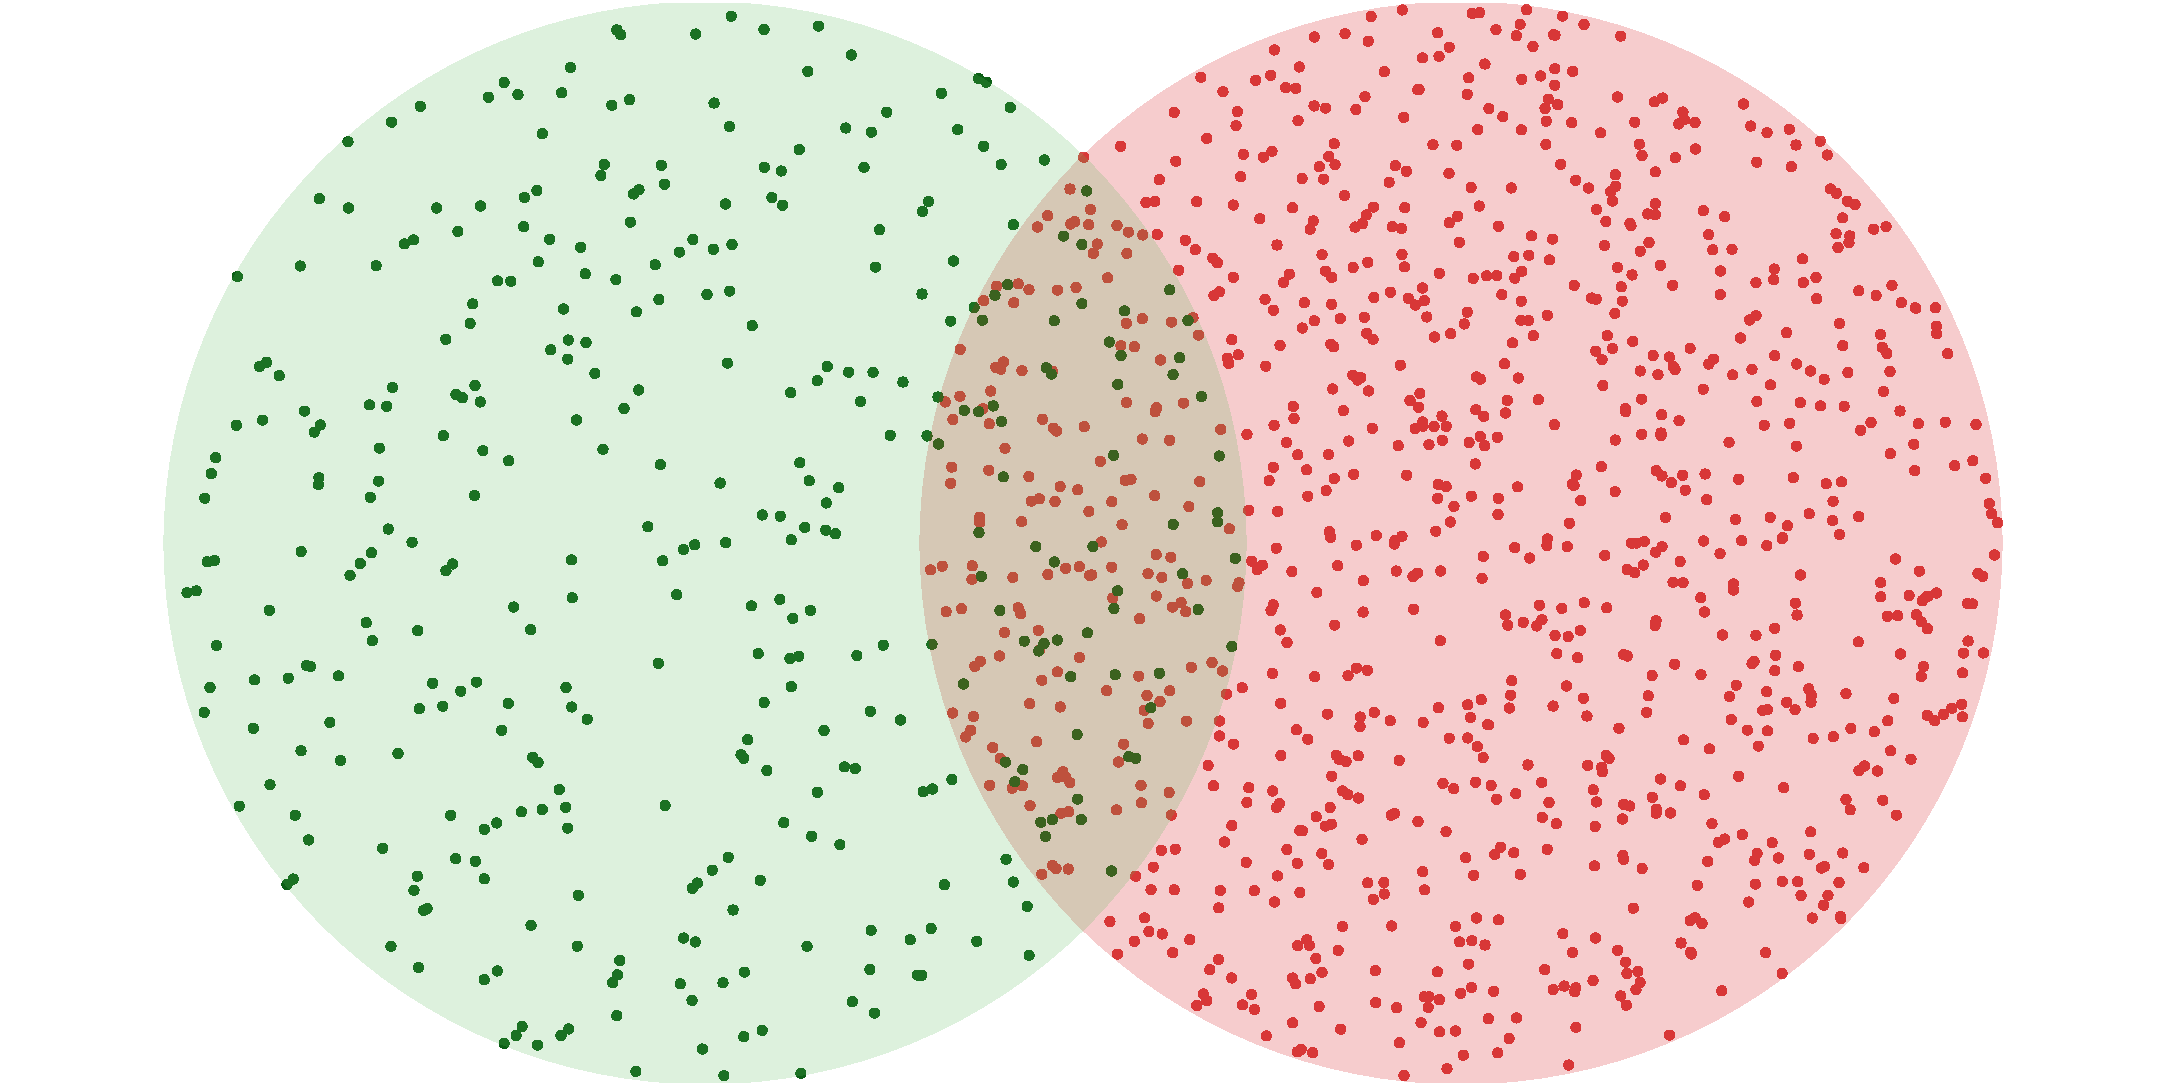
\includegraphics[width=0.22\textwidth]{figs/diagram/Quantative_Simul_Mean=0.0.pdf}
	}
	\subfloat[$(0.26, 57.8\%, 96.9)$]{ 
		\label{fig:diagram 3 group 1}  
		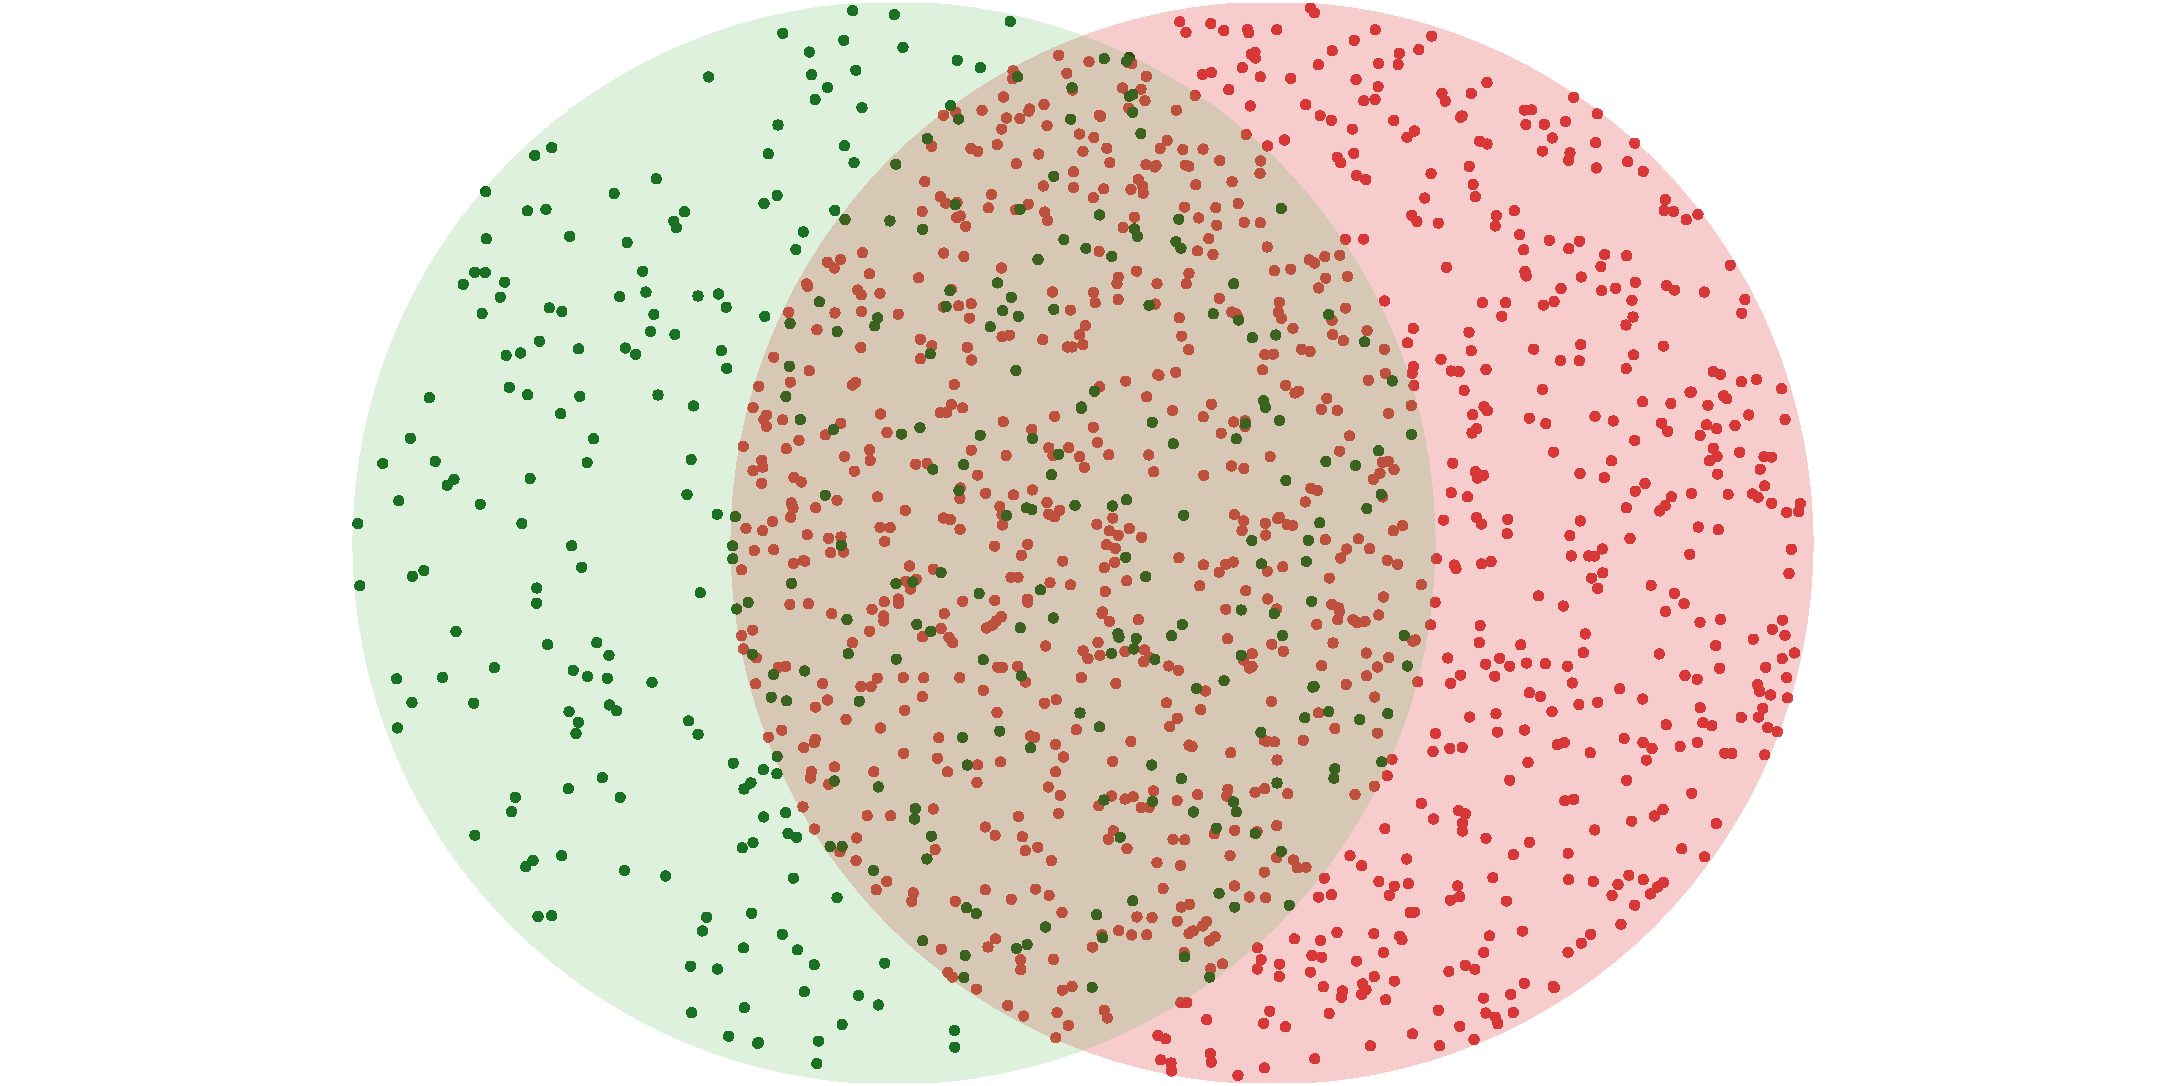
\includegraphics[width=0.22\textwidth]{figs/diagram/Quantative_Simul_Mean=0.7.pdf}
	}
	\subfloat[$(0.05, 100\%, 344.9)$]{
		\label{fig:diagram 4 group 1}
		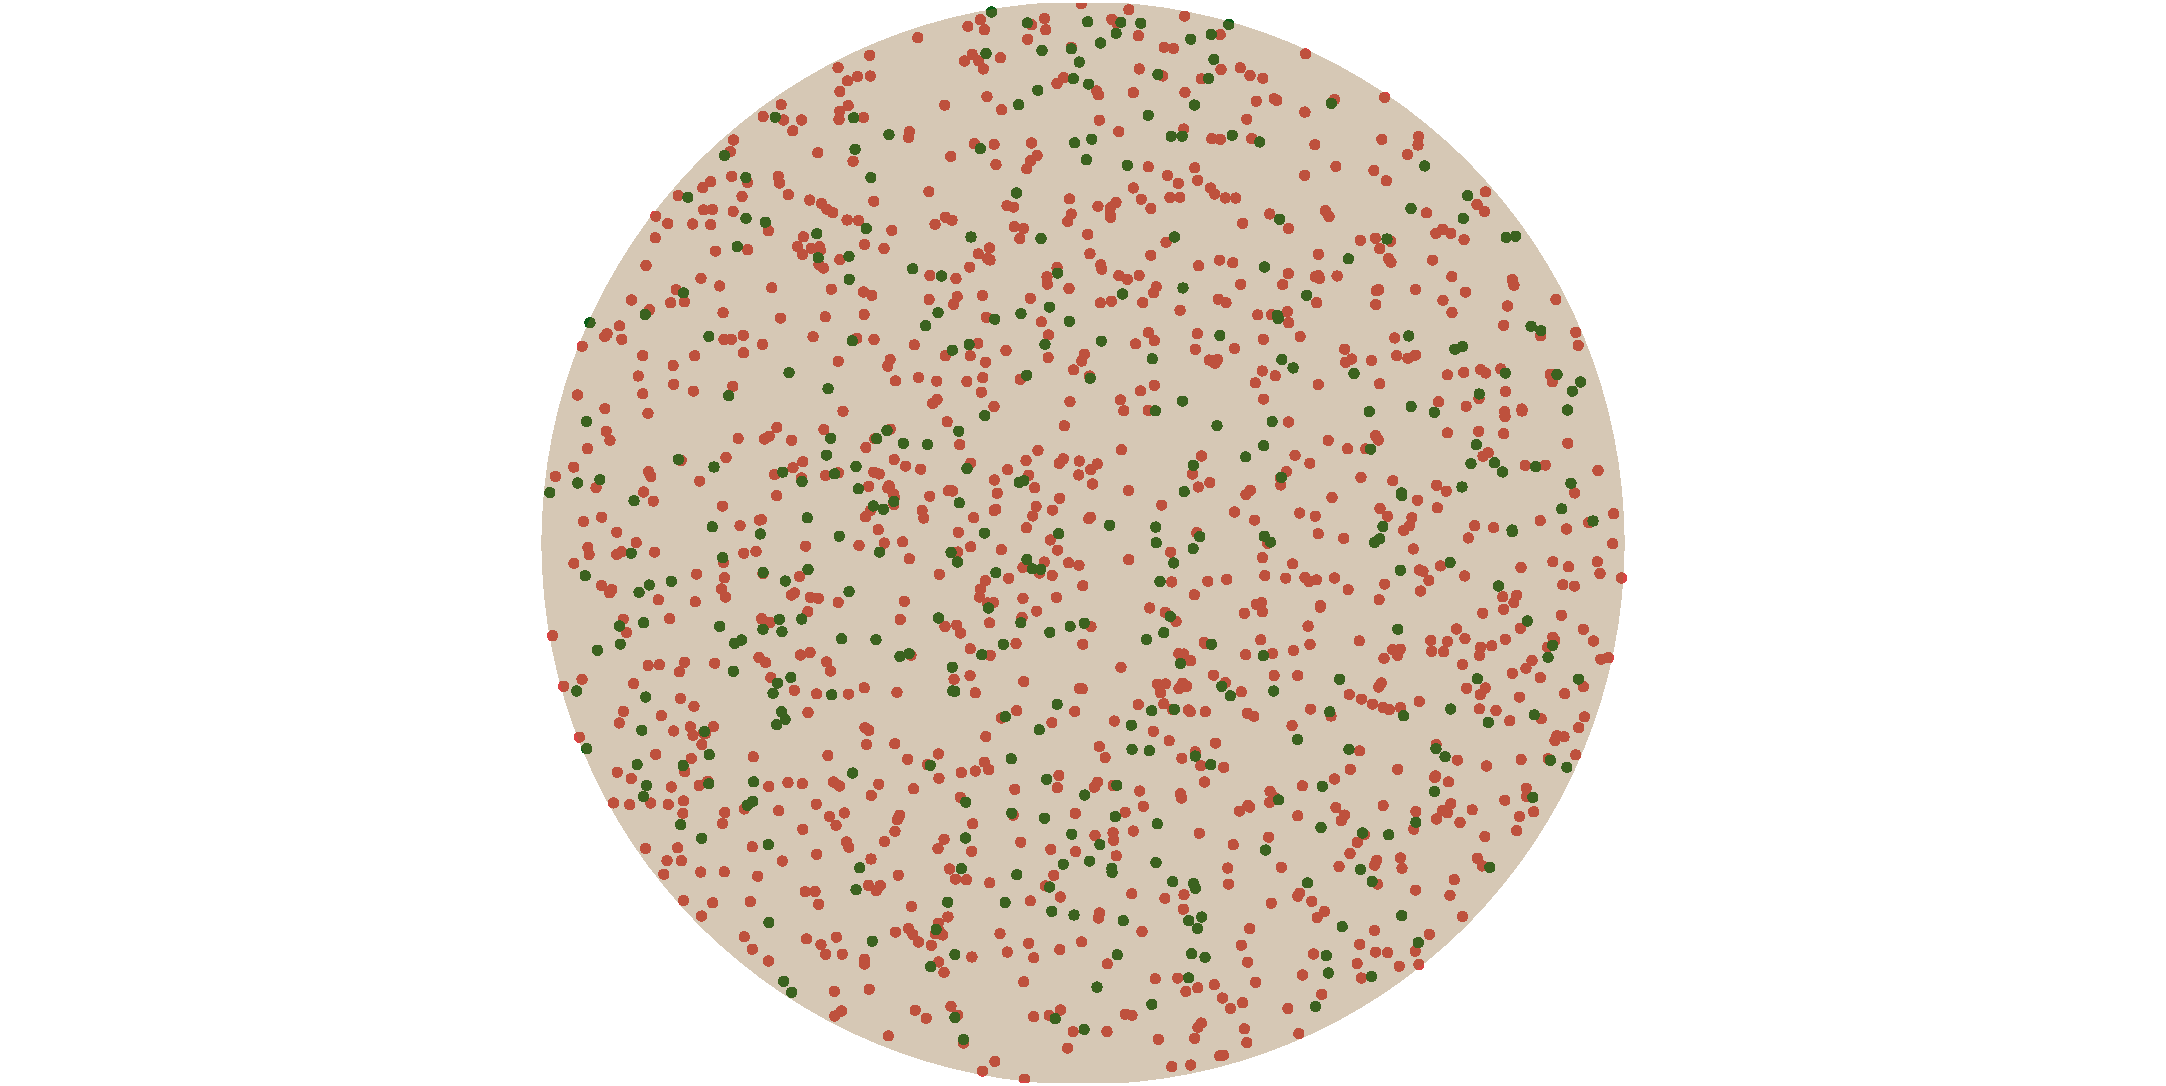
\includegraphics[width=0.22\textwidth]{figs/diagram/Quantative_Simul_Mean=1.4.pdf}
	}
    \vspace{-0.1mm}
	\subfloat[$(0.36, 93.3\%, 63.2)$]{
		\label{fig:diagram 1 group 2}
		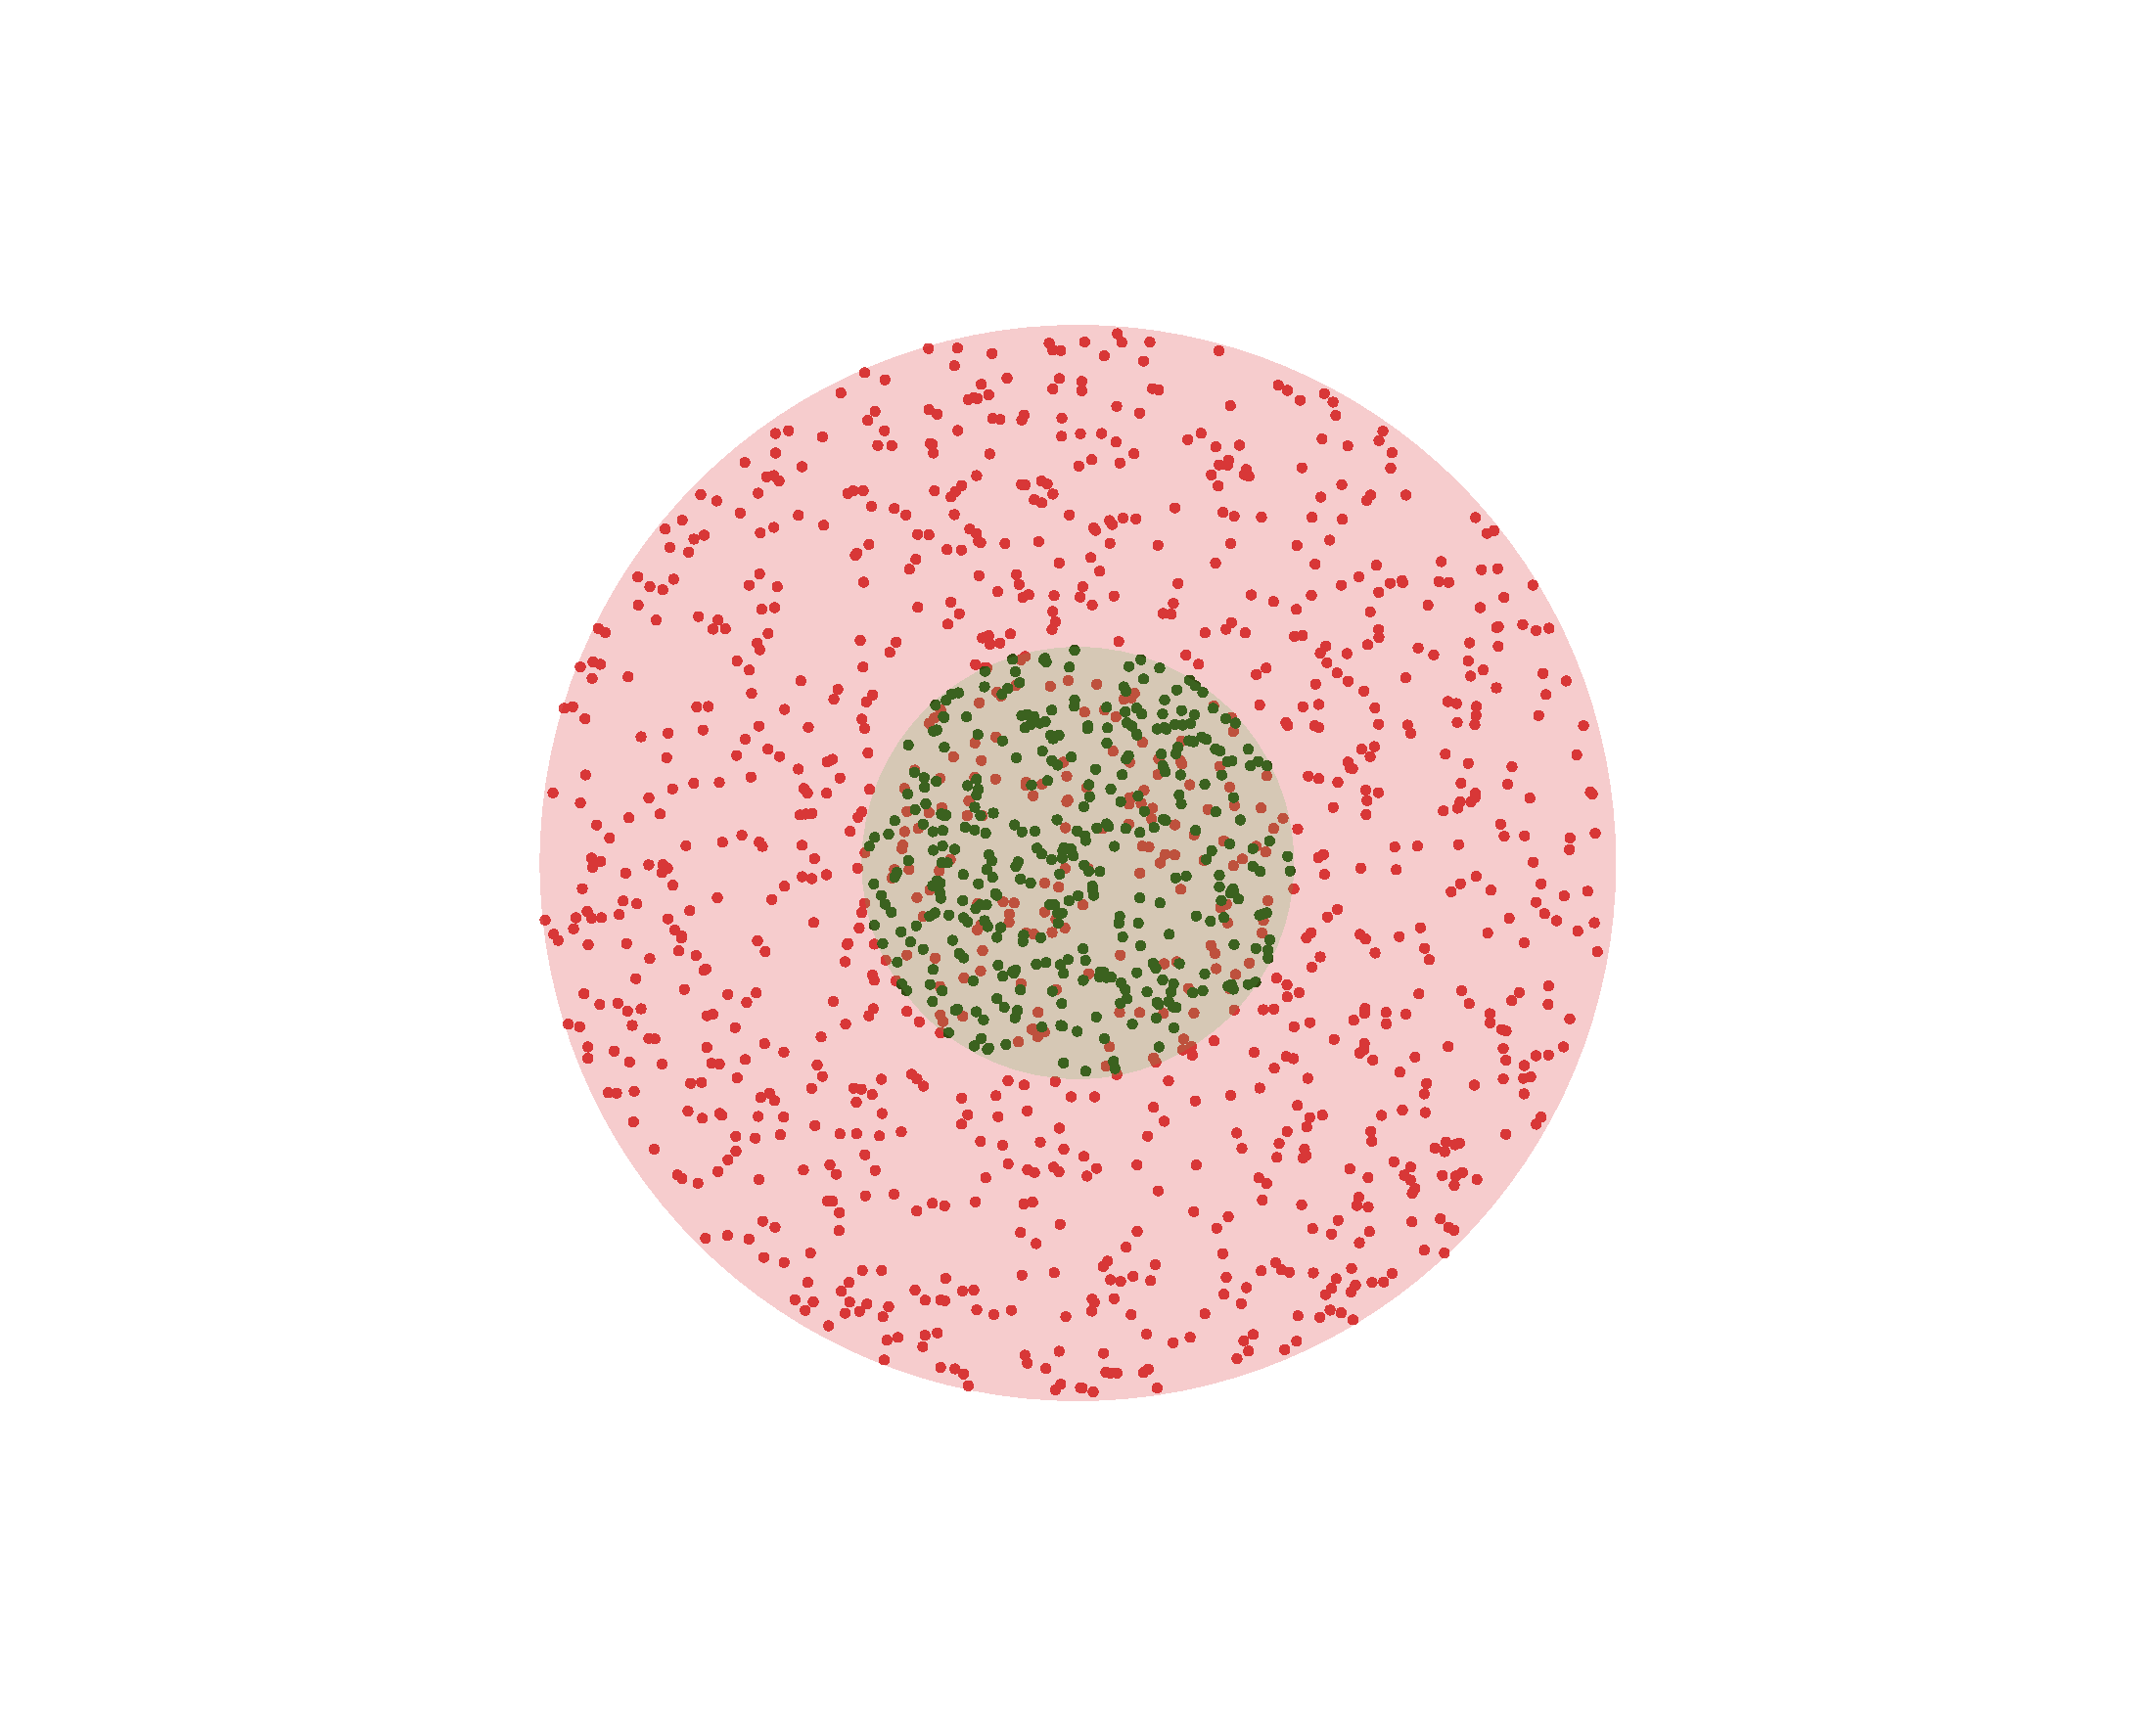
\includegraphics[width=0.22\textwidth]{figs/diagram/Quantative_Simul_R=0.4.pdf}
	}
	\subfloat[$(0.10, 99.8\%, 250.5)$]{
		\label{fig:diagram 2 group 2}
		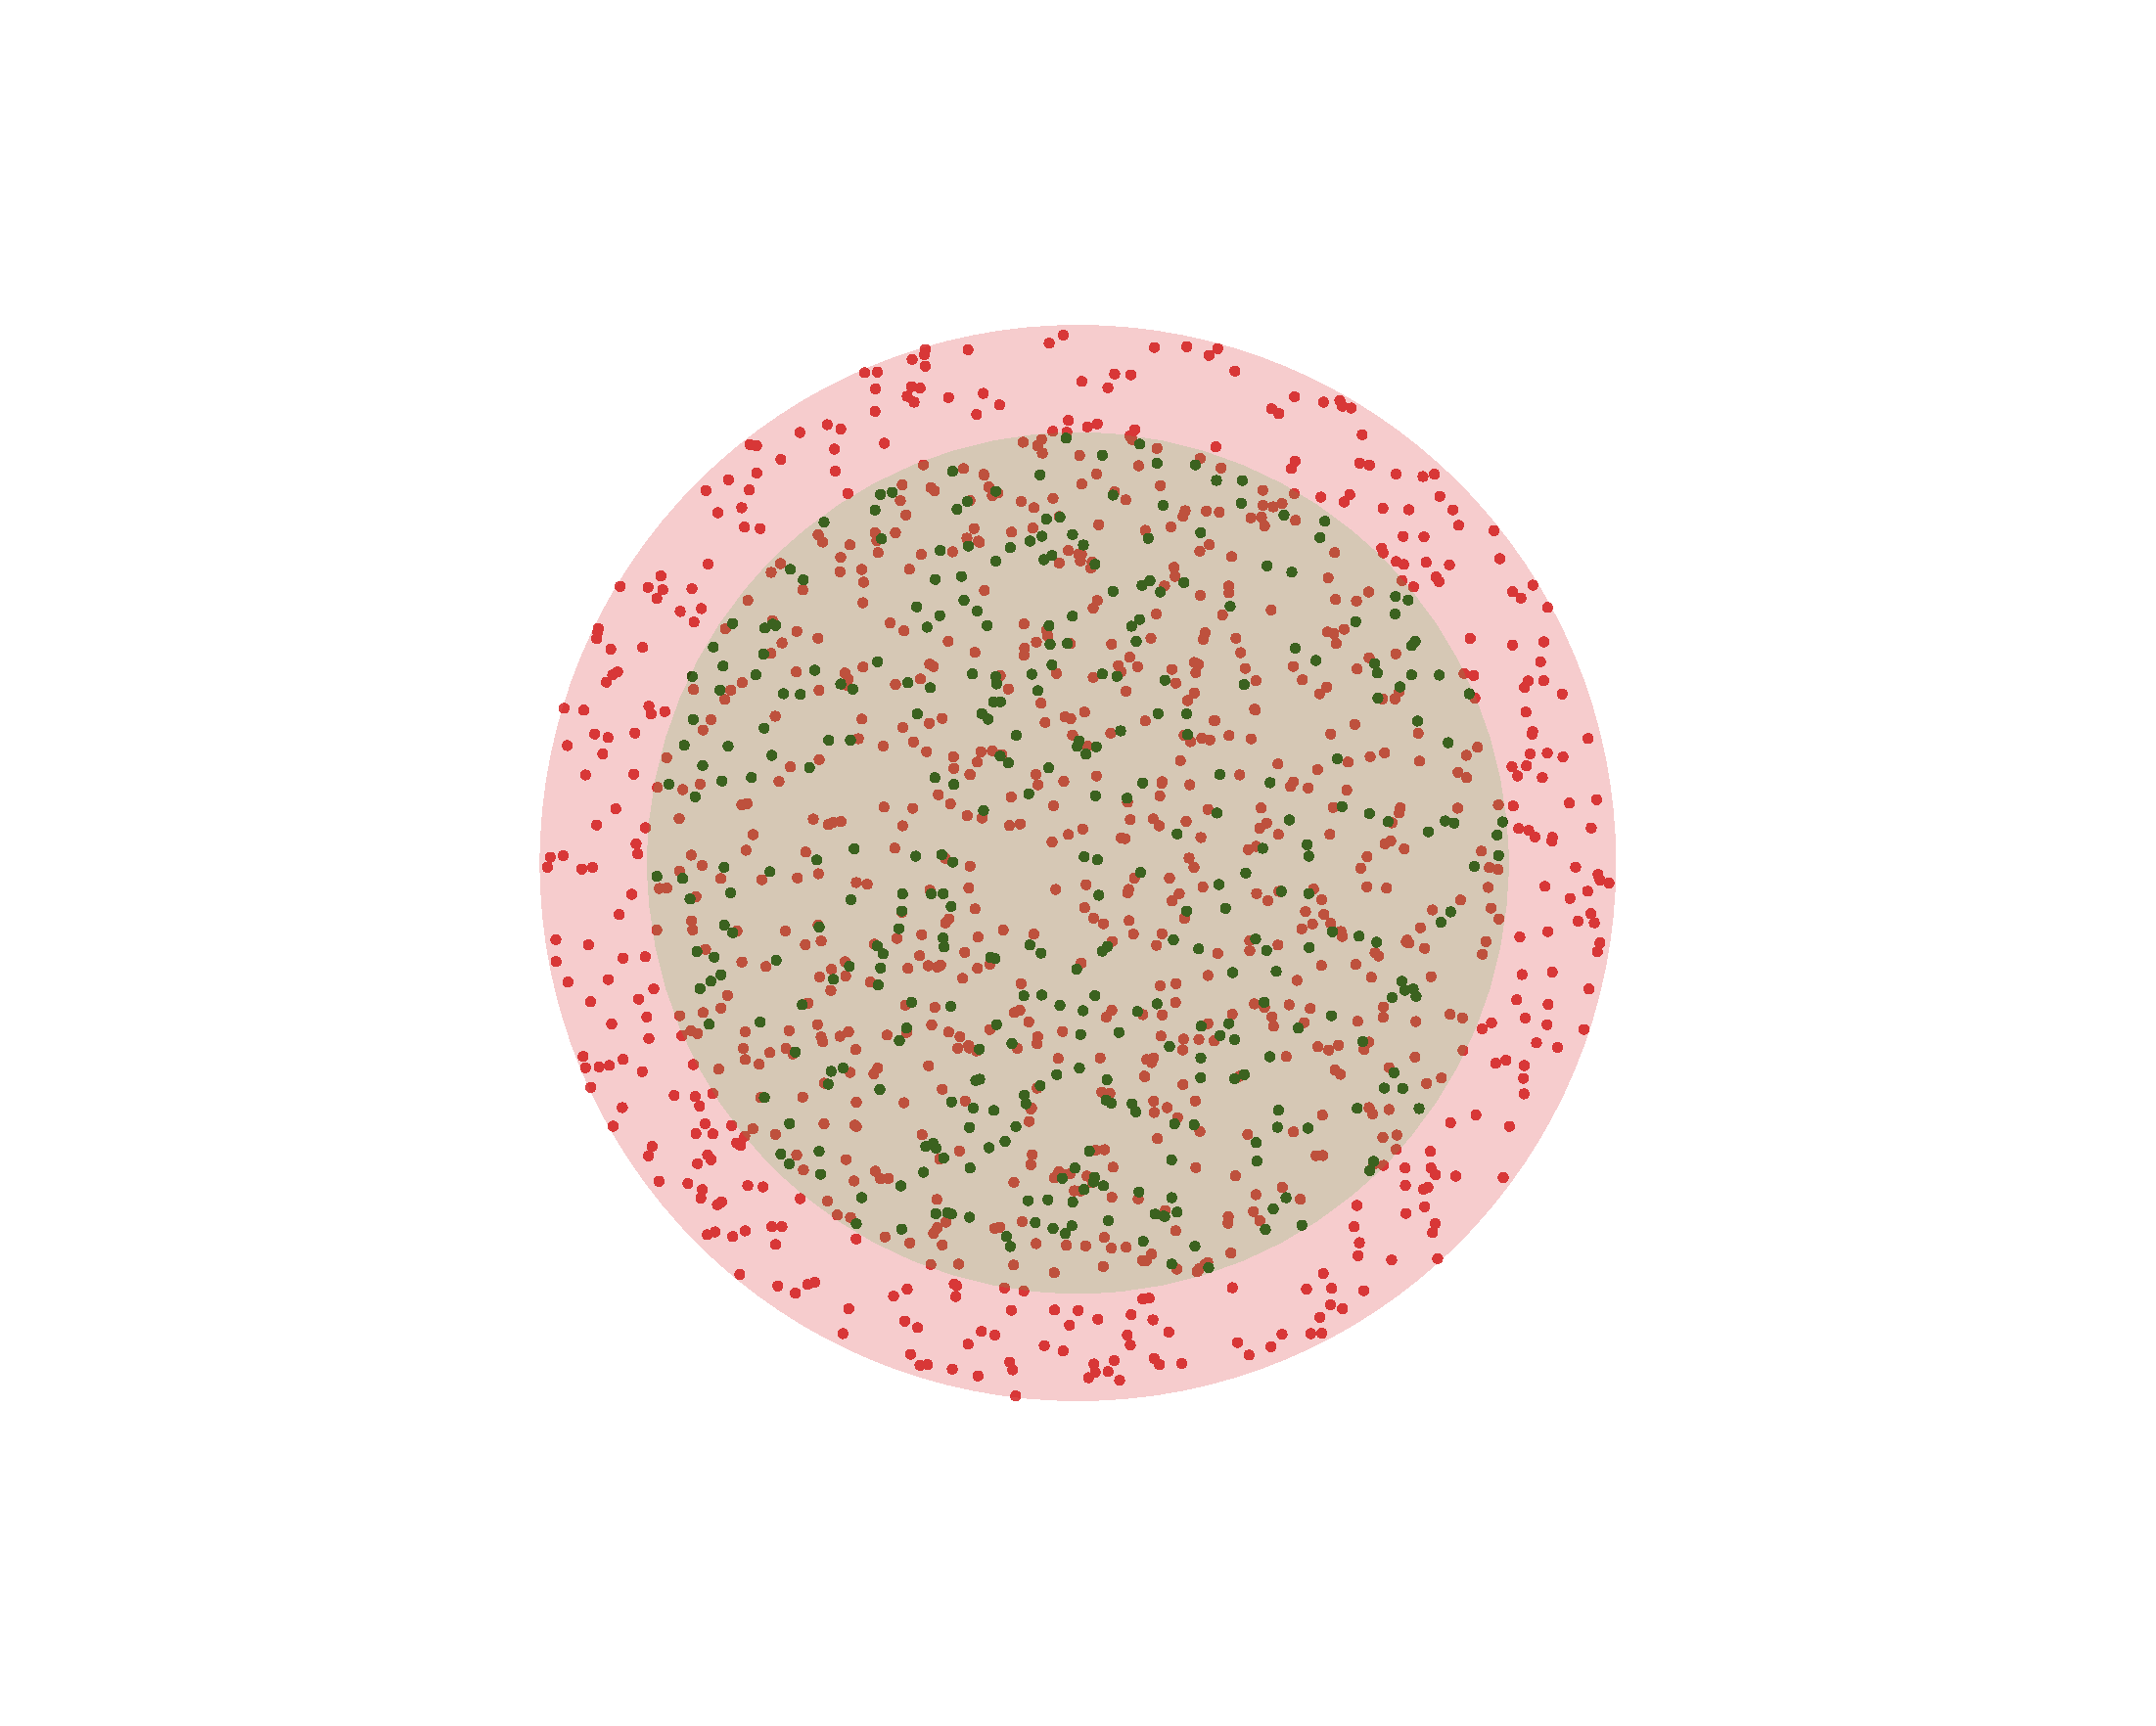
\includegraphics[width=0.22\textwidth]{figs/diagram/Quantative_Simul_R=0.8.pdf}
	}
	\subfloat[$(0.07, 61.3\%, 199.7)$]{
		\label{fig:diagram 3 group 2}
		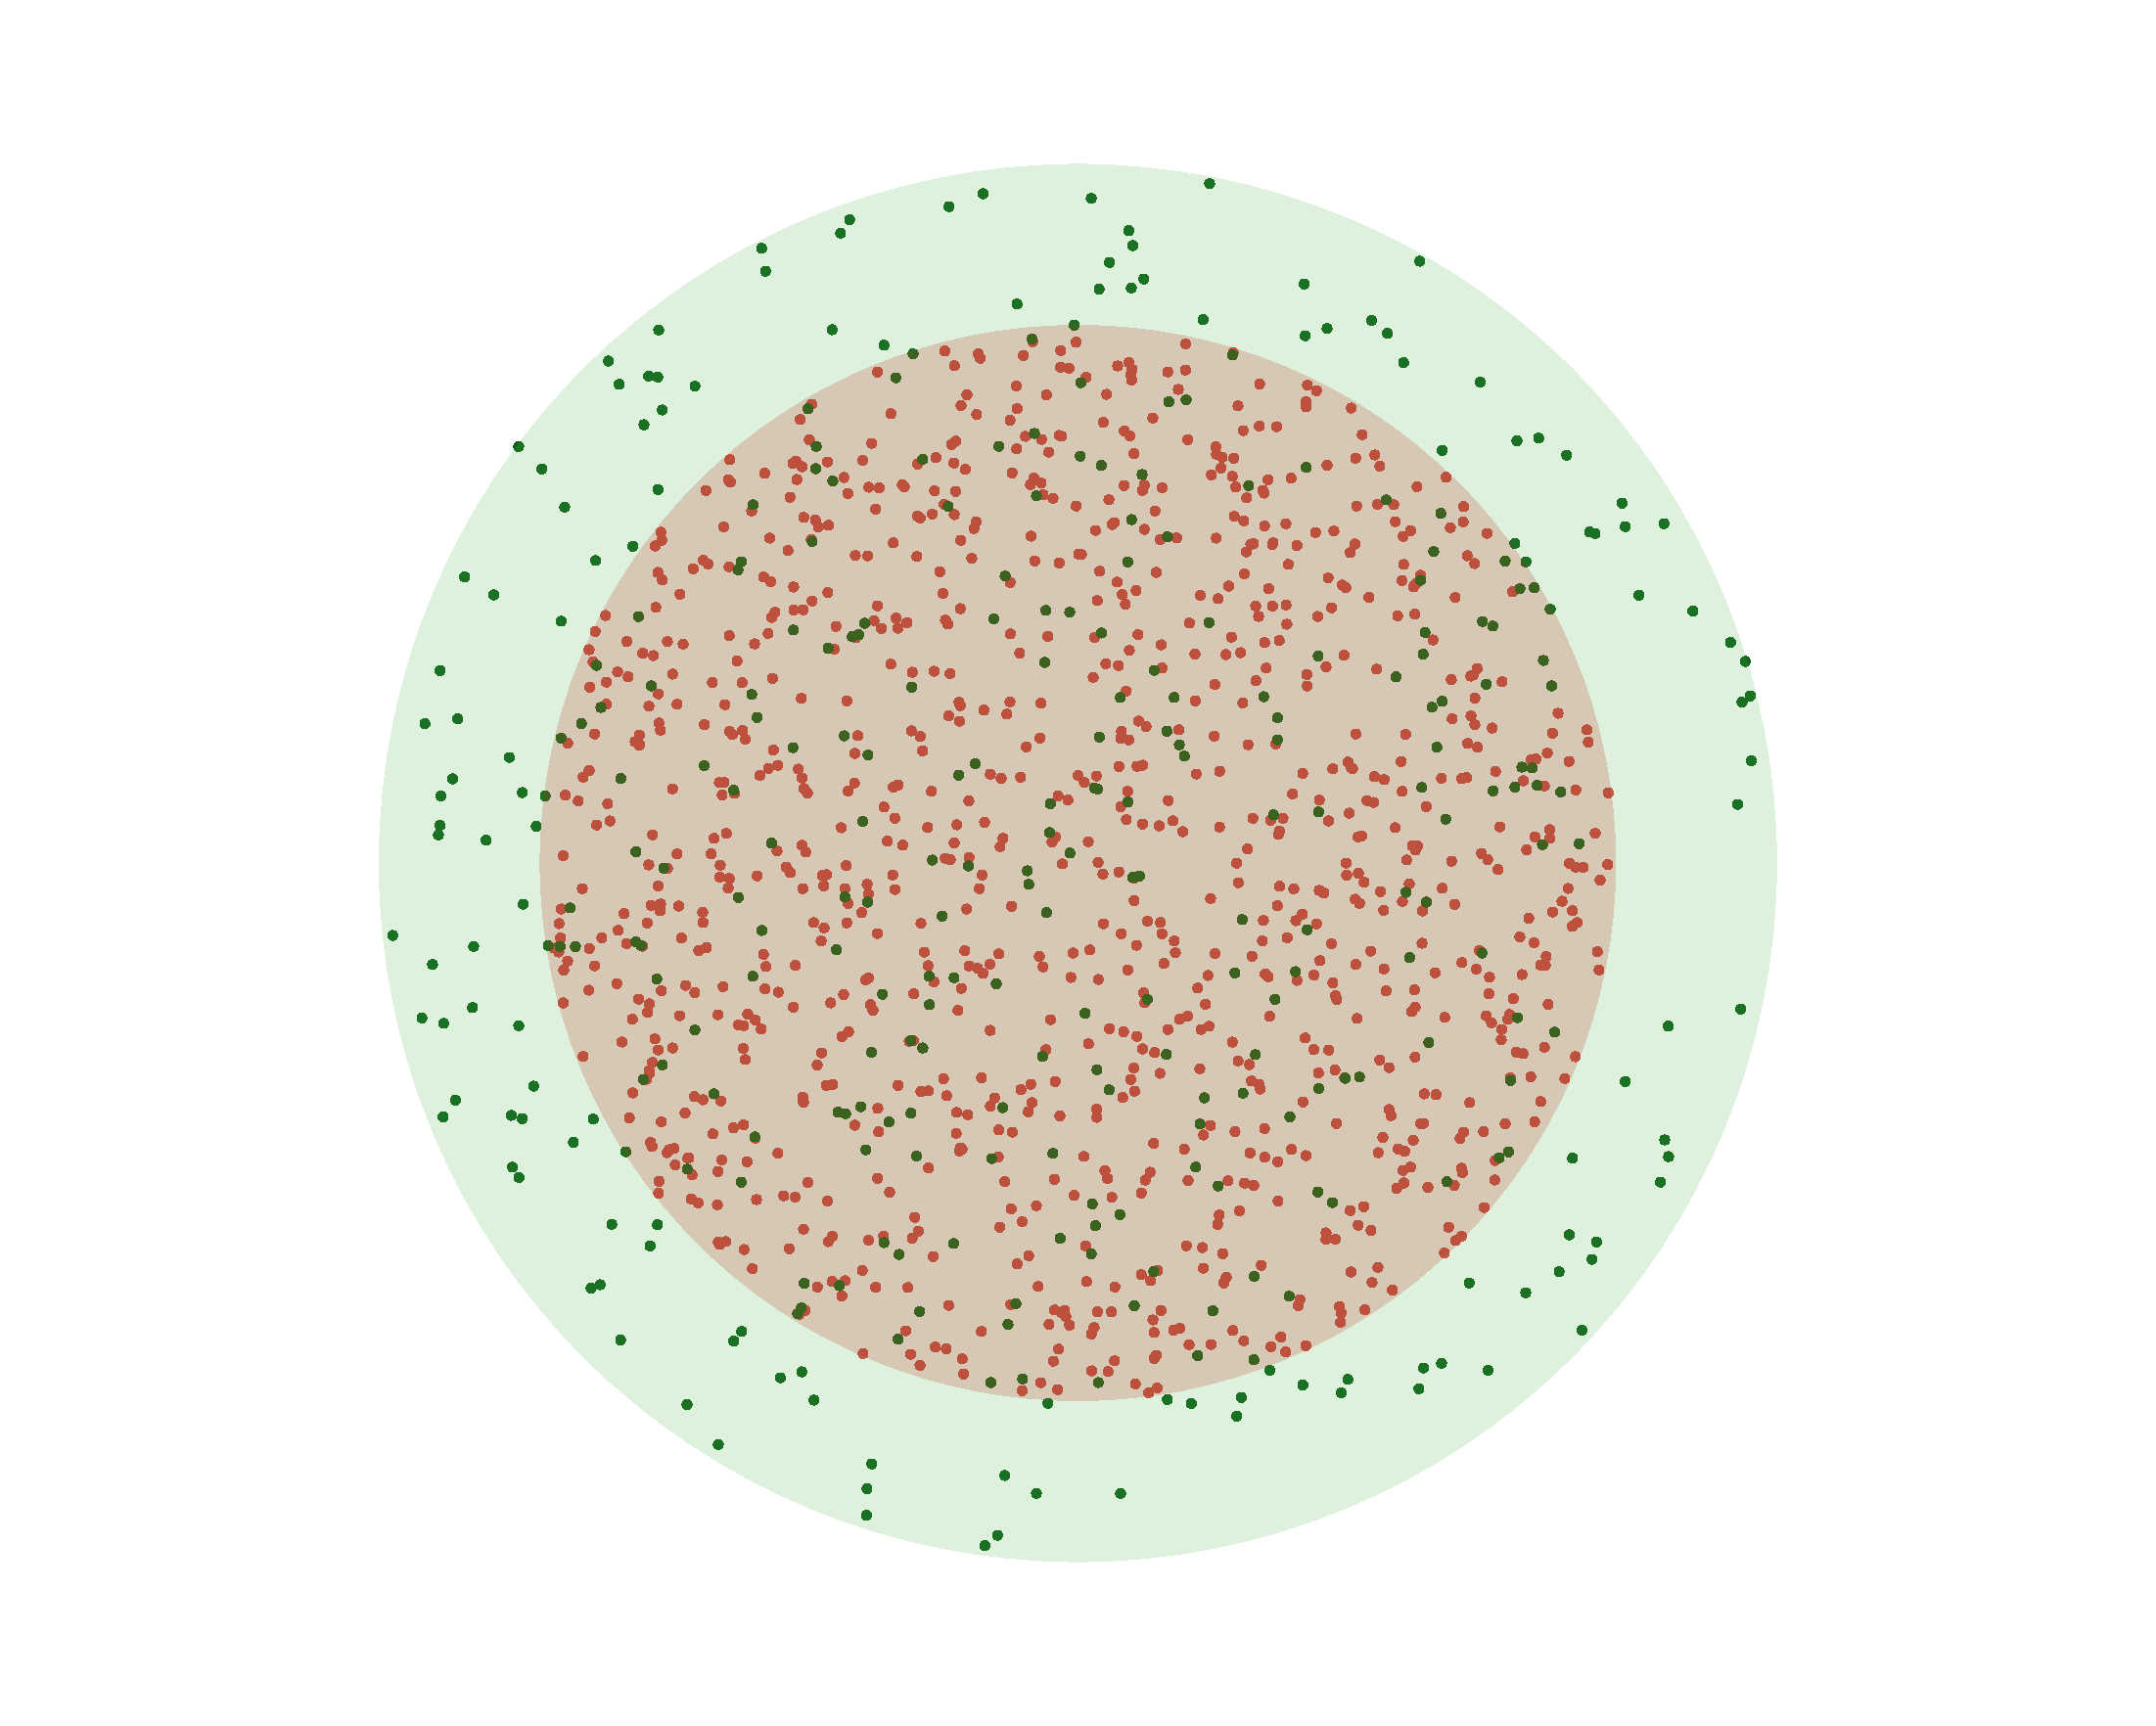
\includegraphics[width=0.22\textwidth]{figs/diagram/Quantative_Simul_R=1.3.pdf}
	}
	\subfloat[$(0.08, 45.3\%, 151.5)$]{
		\label{fig:diagram 4 group 2}
		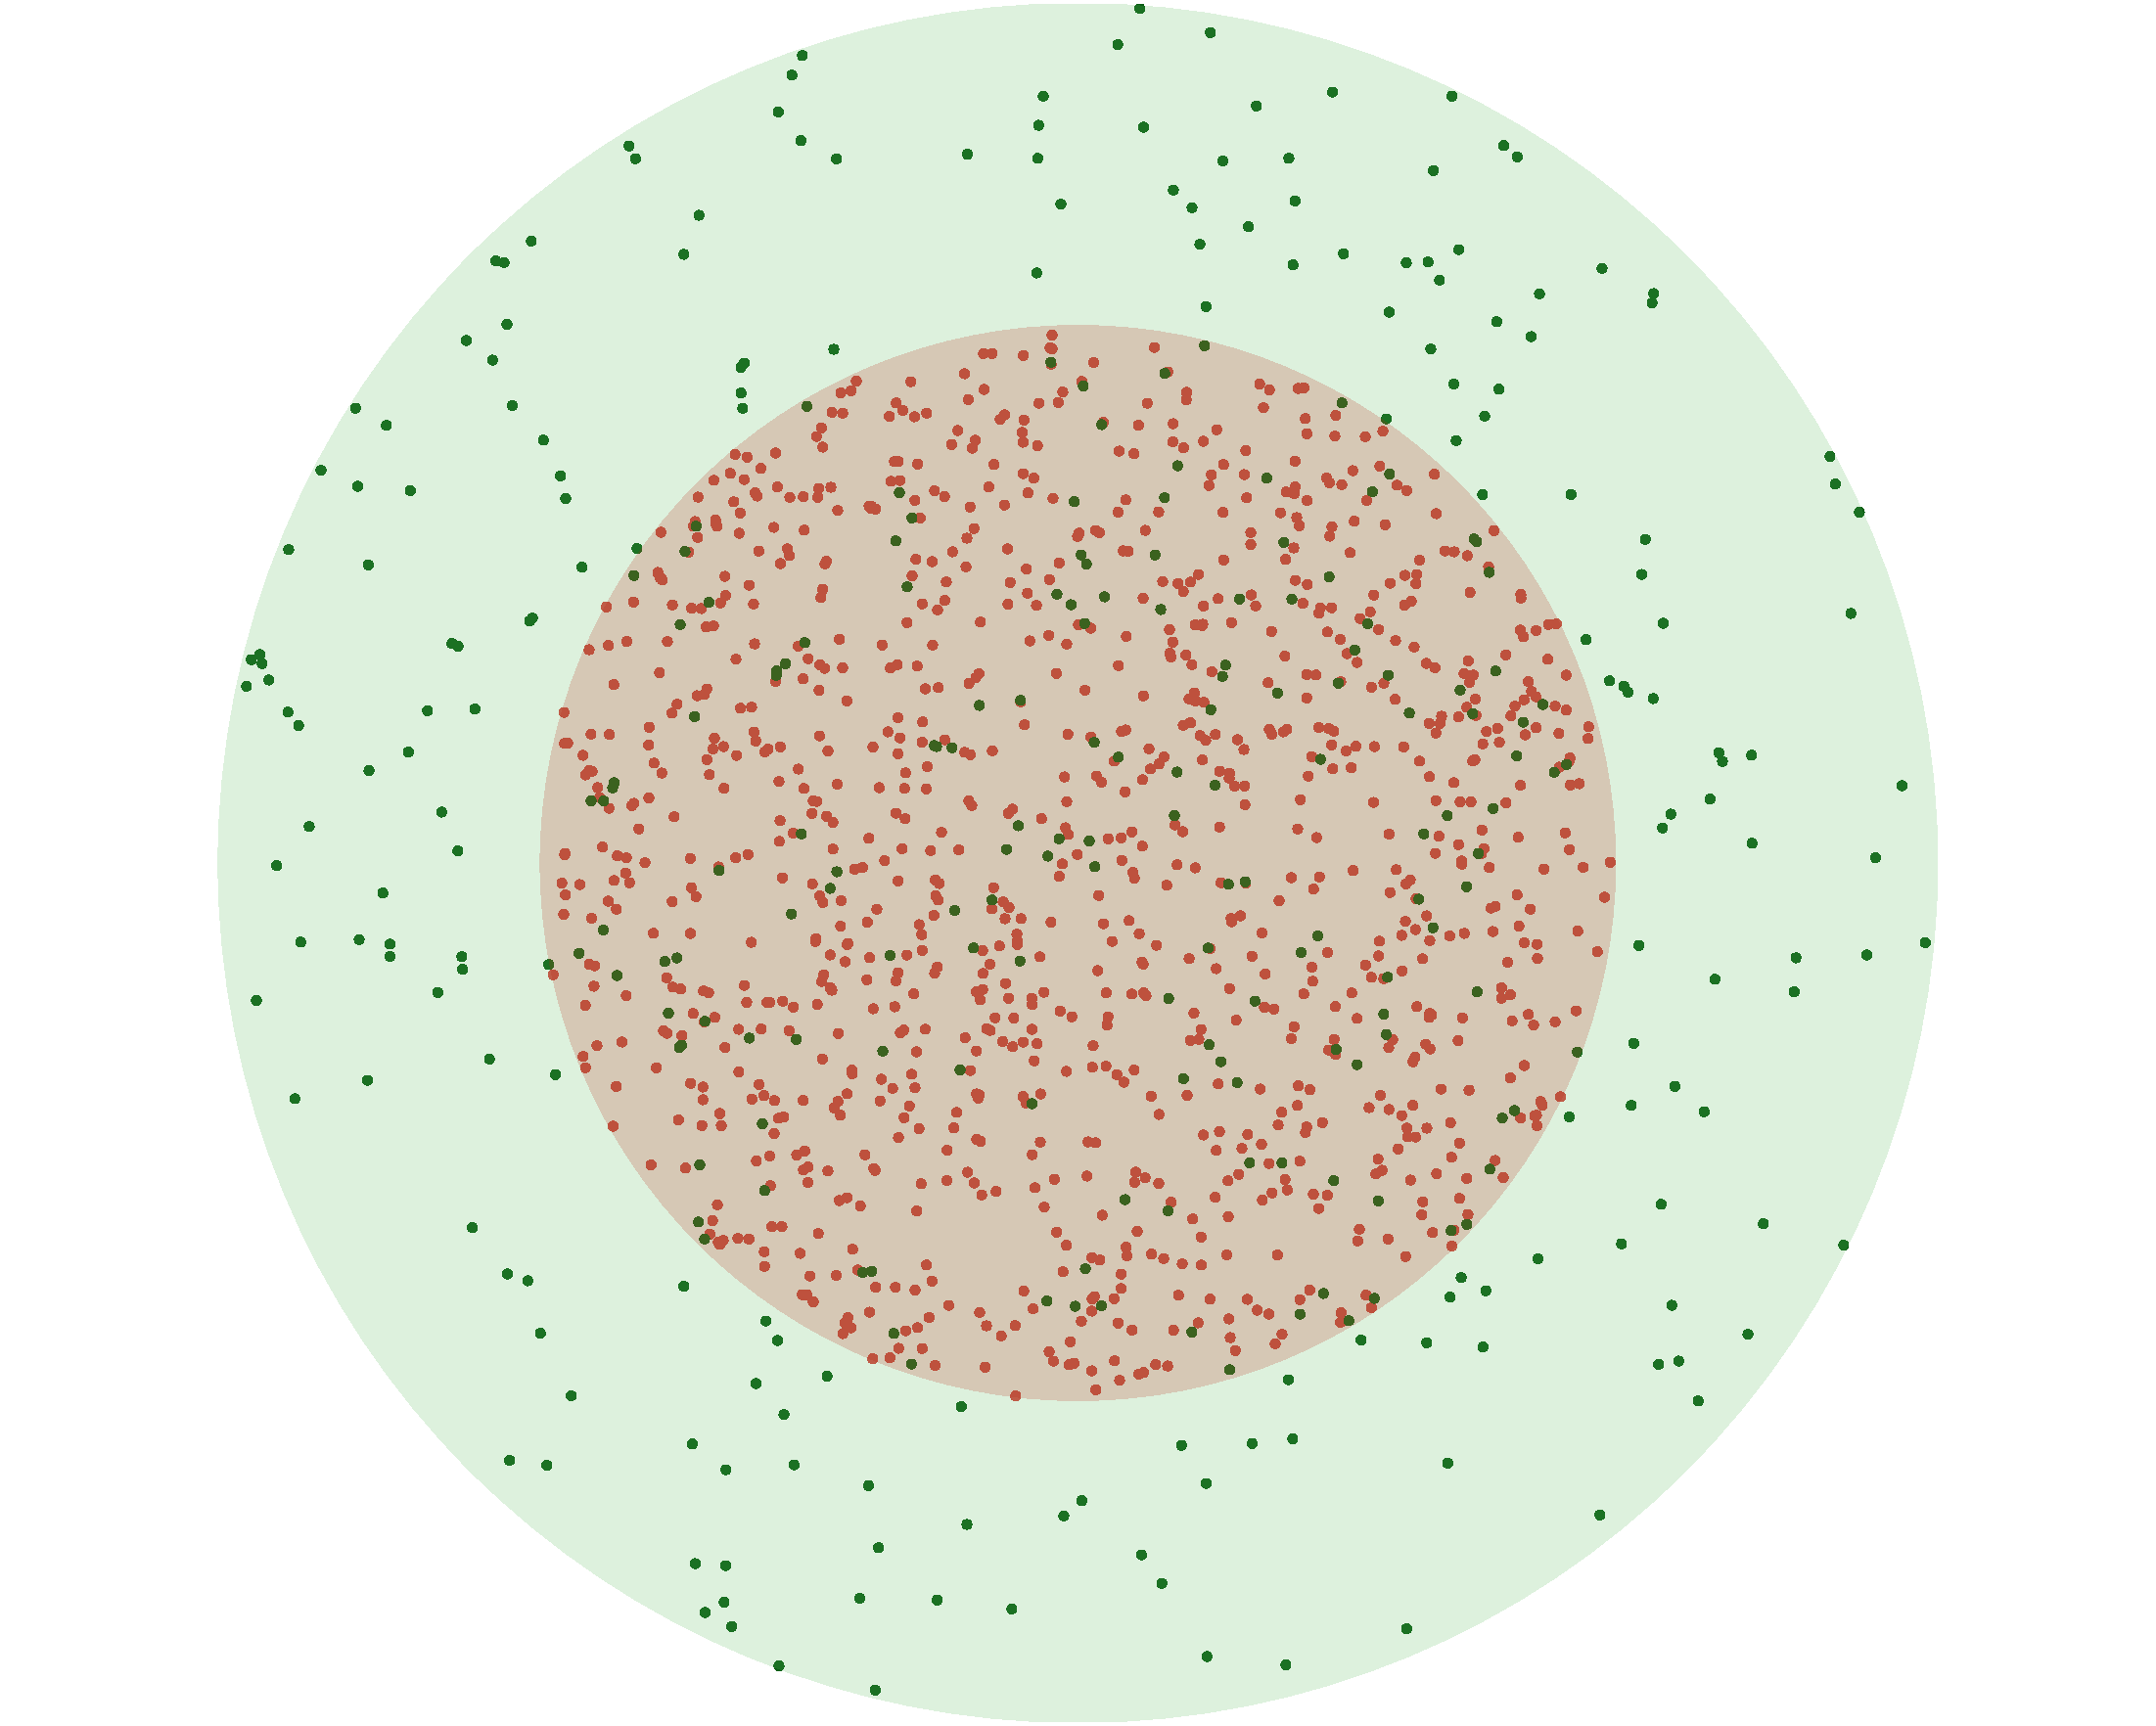
\includegraphics[width=0.22\textwidth]{figs/diagram/Quantative_Simul_R=1.6.pdf}
	}
    \vspace{-1mm}
	\caption{Qualitative analyses of the criterion triple $(\cE, \cU, \cC)$: The red and green disks represent the uniform distributions of feature and code vectors, respectively.}
	\label{fig:criterion triple analysis}
    \vspace{-5mm}
\end{figure*}

\subsection{Theoretical Analyses} \label{sec:theoretical analysis}

In this section, we provide theoretical evidence to support our empirical observations. 
Let the code vectors $\{\be_k\}_{k=1}^K$ and  feature vectors $\{\bz_i\}_{i=1}^N$ be independently and identically drawn from $\cP_B$ and $\cP_A$, respectively.
We say a codebook $\{\be_k\}_{k=1}^K$ attains full utilization asymptotically with respect to  $\{\bz_i\}_{i=1}^N$ if the codebook utilization rate $\cU(\{\be_k\}_{k=1}^K;\{\bz_i\}_{i=1}^N)$ tends to 1 in probability as $N$ approaches infinity:
\begin{align}
\cU(\{\be_k\}_{k=1}^K;\{\bz_k\}_{i=1}^N)\overset{p}{\to}1,\quad \textnormal{as }N\to\infty.
\end{align}
For the codebook distribution $\cP_B$, we say it attains full utilization asymptotically with respect to $\cP_A$ if, with probability 1, the randomly generated codebook $\{\be_k\}_{k=1}^K$ achieves full utilization asymptotically. 


Additionally, a codebook distribution $\cP_B$ is said to have vanishing quantization error asymptotically with respect to a domain $\Omega\subseteq\RR^d$ if the quantization error over all data of size $N$  tends to zero in probability as $K$ approaches infinity:
\begin{align}\label{equ:W25}
\sup_{\{\bz_i\}\subseteq\Omega}\cE(\{\be_k\}_{k=1}^K;\{\bz_i\}_{i=1}^N)\overset{p}{\to}0,\quad \textnormal{as }K\to\infty.
\end{align}
Our first theorem shows that $\overline{\supp(\cP_A)}=\overline{\supp(\cP_B)}$ is sufficient and necessary  for the codebook distribution $\cP_B$ to attain both full utilization and vanishing quantization error asymptotically. For simplicity, $\cP_A$ is assumed to have a density function $f_A$ with bounded support $\Omega\subseteq\RR^d$. 

\begin{theorem}\label{thm:1}
    Assume $\Omega=\supp(\cP_A)$ is a bounded open area. The codebook distribution $\cP_B$ attains full utilization and vanishing quantization error asymptotically if and only if $\overline{\supp(\cP_B)}=\overline{\supp(\cP_A)}$, where $\overline{\cS}$ denotes the closure of the set $\cS$.
\vspace{-1ex}
\end{theorem}
Theorem \ref{thm:1} establishes the optimal support of the codebook distribution. The boundedness of $\Omega$ is required as we consider the worst case quantization error in \eqref{equ:W25}. In real applications, when $\cP_A$ follows an absolutely continuous distribution over an unbounded domain, then $\{z_i\}_{i=1}^N$ generated from $\cP_A$ will be bounded with high probability. Thus, Theorem \ref{thm:1} also provides theoretical insights for a target distribution $\cP_A$ with an unbounded domain.


Besides the optimal support, we also determine the optimal density of the codebook distribution by invoking existing results characterizing asymptotic optimal quantizers \cite{graf2000foundations}. Specifically, we consider the case where $N$ approaches to infinity and define the expected quantization error of a codebook $\{\be_k\}$ with respect to $\cP_\cA$ as 
\begin{align}
\cE(\{\be_k\}_{k=1}^K;\cP_A)=\EE_{\bz\sim\cP_A}\min_{\be\in\{\be_k\}}\norm{\bz-\be}^2.
\end{align}
A codebook $\{\be^*_k\}_{k=1}^K$ is called the set of optimal centers for $\cP_A$ if it achieves the minimal quantization error:
\begin{align}
\cE(\{\be^*_k\}_{k=1}^K;\cP_A)=\min_{\{\be_k\}_{k=1}^K}\cE(\{\be_k\}_{k=1}^K;\cP_A).
\end{align}
Intuitively, Theorem~\ref{thm:1} shows that mismatched supports inevitably lead to either unused code vectors or large quantization error, whereas matching supports is both necessary and sufficient to avoid these failure modes.

Theorem \ref{thm:2} demonstrates that,  under weak regularity conditions,  the empirical measure of the optimal centers for $\cP_A$ converges in distribution to a fixed distribution determined by $\cP_A$. Notably, we do not assume a bounded domain in the following theorem.


\begin{theorem}[Theorem 7.5, \cite{graf2000foundations}]\label{thm:2} 
Suppose $Z\sim\cP_A$ is absolutely continuous w.r.t. the Lesbegue measure in $\RR^d$ and $\EE\norm{Z}^{2+\delta}<\infty$ for some $\delta>0$.
Then the empirical measure of the optimal centers for $\cP_A$, 
\begin{align}
\frac{1}{K}\sum_{k=1}^K\delta_{\be^*_k},
\end{align}
converges weakly to a fixed distribution $\cP_A^*$, whose density function $f_A^*$ is proportional to $f_A^{(d+2)/d}$. 
\end{theorem}


% together with the Glivenko-Cantelli theorem \cite{van1996weak},\scomment{how does this "together with GC"? I think Theorem 2 already uses GC somehow?}
 
% Theorem \ref{thm:2} implies that $\cP_B=\cP_A^*$ is the optimal codebook distribution in the asymptotic regime as $K$ approaches infinity. In high-dimensional spaces with large $d$, this optimal  distribution $\cP_B=\cP_A^*$ closely approximates $\cP_A$. This further motivates us to align the codebook distribution $\cP_B$ with the feature distribution $\cP_A$. 

% \textcolor{green}{\paragraph{High-dimensional implication.}
% Theorem~\ref{thm:2} characterizes the asymptotically optimal codebook distribution $\cP_A^*$, whose density satisfies
% $f_A^*(z)\propto f_A(z)^{(d+2)/d}$.
% A key implication arises in high-dimensional settings: as $d$ grows, the exponent approaches one,
% \begin{align}
% \lim_{d\to\infty} \frac{d+2}{d} = \lim_{d\to\infty} \left(1+\frac{2}{d}\right) = 1.
% \end{align}
% so $f_A^*$ becomes increasingly close to $f_A$.
% Equivalently, the optimal codebook distribution $\cP_A^*$ approaches the feature distribution $\cP_A$ in the high-dimensional regime.
% Since visual tokenization typically uses moderately to high-dimensional latent features (e.g., $d$ in common VQ-based tokenizers is on the order of hundreds), this provides additional theoretical support for explicitly aligning the codebook distribution with the feature distribution, i.e., $\cP_B \approx \cP_A$. This observation motivates our distributional matching objective, which explicitly encourages $\cP_B$ to track $\cP_A$ as a practical surrogate for the asymptotically optimal design.}

% \textcolor{red}{\paragraph{High-dimensional Implication.}
% Theorem~\ref{thm:2} characterizes the asymptotically optimal codebook distribution $\mathcal{P}^*_A$, whose density satisfies $f^*_A(z) \propto f_A(z)^{(d+2)/d}$. 
% A critical implication arises in high-dimensional settings typical of visual tokenization (e.g., $d \ge 256$): as the dimension $d$ grows, the exponent converges to unity,
% \begin{align}
% \lim_{d\to\infty} \frac{d+2}{d} = \lim_{d\to\infty} \left(1+\frac{2}{d}\right) = 1.
% \end{align}
% Consequently, the optimal codebook density $f^*_A$ converges exactly to the feature density $f_A$.
% This mathematical insight provides a rigorous foundation for our approach: in the high-dimensional regime, explicitly aligning the codebook distribution with the feature distribution (i.e., $\mathcal{P}_B \approx \mathcal{P}_A$) yields the theoretically optimal VQ solution.
% This observation legitimizes our distributional matching objective, which encourages $\mathcal{P}_B$ to track $\mathcal{P}_A$ as a highly accurate practical surrogate for the asymptotically optimal design.}
\paragraph{High-dimensional Implication.}
Theorem~\ref{thm:2} characterizes the asymptotically optimal codebook distribution $\mathcal{P}^*_A$, whose density satisfies
$f^*_A(z) \propto f_A(z)^{(d+2)/d}$.
A key implication arises in high-dimensional settings typical of visual tokenization: as the feature dimension $d$ increases, the exponent converges to unity,
\begin{align}
\lim_{d\to\infty} \frac{d+2}{d} = \lim_{d\to\infty} \left(1+\frac{2}{d}\right) = 1.
\end{align}
As a result, the optimal codebook density $f^*_A$ becomes increasingly close to the feature density $f_A$ in the high-dimensional regime.
This observation provides a rigorous theoretical justification for our approach: explicitly aligning the codebook distribution with the feature distribution (i.e., $\mathcal{P}_B \approx \mathcal{P}_A$) serves as a principled and effective surrogate for the asymptotically optimal design in high-dimensional latent spaces.


%Theorem \ref{thm:2} implies that in the asymptotic regime where $K\to\infty$,    

%\paragraph{Summary} Our theoretical evidence closely aligns with our empirical findings, reinforcing the claim that optimal VQ can be achieved when $\cP_B$ is identical to $\cP_A$, which implies that $\mathcal{M}_{\lambda_2=0}$ achieves its minimum.
